\graphicspath{{lit_study/fig/}}

{
\tikzset{external/figure name/.add={lit_study/}{}}


\chapter{Literature study}
\label{chap:lit_study}

\section{Payload transportation with multirotors}

    \paragraph
    The transportation of payloads with \glspl{UAV} has significantly grown in popularity over recent years.
    % Examples of specific applications of \gls{UAV} transportation include package deliveries \cite{}, pesticide application in agriculture \cite{}, and 
    Multirotor \glspl{UAV} are specifically useful for many transportation applications due to their agility, and their \gls{VTOL} and hover capabilities.
    The types of payloads attached to multirotors can usually be categorised as either sensors (e.g. cameras and meteorological sensors), or freight (e.g. mail parcels or fire extinguishing material) \cite{Vergouw2016}.
    Furthermore, the payload attachment is mainly categorised as either a rigid connection, or a cable-suspended connection \cite{Vergouw2016}.
    In rare cases, a robotic actuator is attached to the multirotor to manipulate the payload \cite{Gonzalez-deSantos2020} \cite{Suthar2021}.
    The payload attachment and the physical properties of the payload influence the flight dynamics of a multirotor and needs to be considered for control system design.   
    In many applications, some aspects of the payload configuration are unknown prior to flight and the control architecture needs to account for these unknowns.

    % figure of rigid and suspended payload

    \subsection{Rigidly attached payloads}

        \paragraph
        Payloads are often rigidly attached to a multirotor for transportation.
        This configuration is especially popular for commercial package deliveries \cite{San2018}.
        There is minimal relative movement between the multirotor and the rigidly connected payload, hence, the payload only affects the \gls{CoM}, the moment of inertia, and the aerodynamics of the vehicle.
        Often, the weight and size of the payload is unknown prior to flight.
        
        \paragraph
        Different control approaches have been proposed to deal with the altered flight dynamics for this applications, 
        including \gls{ARC} \cite{Min2011} and \gls{MRAC} \cite{Emran2015}.
        These control architectures mostly involve a parameter estimation algorithm to estimate the inertial parameters,
        and an adaptive control law which is based on the estimated parameters and a dynamical model of the system.

        % \paragraph
        % \author{Mellinger2011a} \cite{Mellinger2011a} proposed an adaptive controller for a multirotor with a rigidly connected payload.
        % Least-squares estimation techniques were applied to estimate the inertial parameters of the payload.
        % A adaptive control law was then applied which uses the estimated parameters in the control law.
        % Experimental results showed acceptable trajectory tracking performance with the adaptive controller.

        \paragraph
        An advantage of rigidly connected payloads is that the flight dynamics are not altered significantly.
        The payload does not add a degree of freedom to the system and only the inertial parameters need to be account for.
        However, this configuration limits the shape and size of a potential payload, since
        the payload needs to be compatible with the vehicle gripper.
        The multirotor also needs to land or approach the payload very closely to attach to the load, which may be impractical in many applications.

    \subsection{Cable-suspended payloads}

        \paragraph
        Figure~\ref{fig:real_suspended_payload_example} shows an example of a practical application of a suspended payload used during search and rescue missions.
        The shape and mass of the payload has an effect on the flight dynamics, but the payload is often unknown prior to flight.
        The control system should be able to account for these uncertainties and fly well despite the altered flight dynamics.

        \begin{figure}[htb]
            \centering
            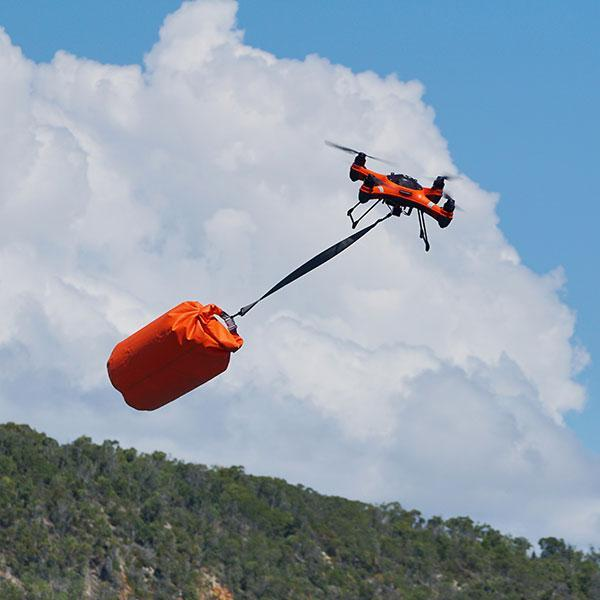
\includegraphics[width=0.45\linewidth]{real_suspended_payload_example.jpg}            
            \caption{A practical suspended payload used for search and rescue missions \cite{CompareCommander2020}}
            \label{fig:real_suspended_payload_example}
        \end{figure}

        \paragraph
        The transportation of various suspended payload configurations have been considered in literature.
        The classical suspended payload application involves a small payload suspended below the vehicle with rigid cable \cite{Guerrero-Sanchez2017} \cite{Klausen2017} \cite{Ichikawa2018} \cite{DeAngelis2019a} \cite{Erasmus2020} \cite{Slabber2020}. 
        \author{Kotaru2017} \cite{Kotaru2017} considered a suspended payload system with an elastic cable modelled as a spring-damper system.
        \author{Tang2015a} \cite{Tang2015a} modelled the multirotor-payload system with a hybrid dynamical model to consider aggressive manoeuvres where the cable transitions from taut to slack.
        The transportation of payload loads with flexible cables have also been studied, where the cable is modelled as a set of serially-connected rigid links  \cite{Goodarzi2015} \cite{Goodarzi2014} \cite{Kotaru2018}. 
        Furthermore, the control of a group of multirotors transporting a single suspended payload have also been considered \cite{Lee2015} \cite{Sanalitro2020} \cite{Klausen2014} \cite{Goodarzi2015}.
        
        \paragraph
        From numerous examples in literature, it is clear that the control of multirotors with suspended payloads is a popular research topic.
        The cable-suspended payload configuration is very useful in situations where a multirotor cannot land, since the payload can be attached during hover.
        This configuration also has the advantage that a load can have an arbitrary shape or size as long as it has an attachment point for a cable.
        However, the suspended payload increases the degrees of underactuation of the system, which makes the control problem challenging \cite{Kotaru2018}.

\section{Control of a multirotor with a suspended payload}

    \subsection{Input shapers}

    \subsection{Active-damping controllers}

    
    % ?? Lit study: include different types of \gls{MPC}, e.g. DMC, MAC
    % ?? different types of models \cite{}, 
    % ?? See \cite{Garcia1989} for good example of different implementations with different models
 

\section{System identification of a multirotor with an unknown suspended payload}

   
% \section{System Design}
% Blok diagram
% komponente

}


